\section{Métodos Preditores-Corretores}

Consistem de dois passos:

\begin{enumerate}
 \item Preditor: estima a solução para um novo ponto.
 \item Corretor: melhora a precisão da estimativa.
\end{enumerate}

\subsection{Introdução}

\begin{figure}[htb]
 \centering
 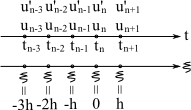
\includegraphics[scale=1.0]{capitulos/capitulo6/figuras/met_pred_corretores1.png}
 \caption{?}
 \label{fig:met_pred_corretores1}
\end{figure}

\begin{equation}
 \label{cap6:sec4:eq1}
 \xi = t - t_n
\end{equation}

Problema:

\begin{equation}
 \label{cap6:sec4:eq2}
 \left\{
 \begin{array}{l}
  u' = f \, (u, \, t) \\
  u \, (0) = u_0
 \end{array}
 \right.
\end{equation}

\begin{equation}
 \label{cap6:sec4:eq3}
 u_{n+1} = u_n + \int_0^h u' \, (\xi) \, d\xi
\end{equation}

Idéia do método:

\begin{itemize}

\item desenvolver uma função de interpolação para \esp{ u' \, (\xi) } baseada em valores de \esp{ u'_i }, em pontos \esp{ t_i, \, i \leq n }, conhecidos.

\item integrar \ref{cap6:sec4:eq3} analiticamente, obtendo uma extrapolação para \esp{ \bar{u}_{n+1} } (preditor).

\item calcular \esp{ \bar{u}'_{n+1} = f \, (\bar{u}_{n+1}, \, t_{n+1}) }

\item desenvolver uma nova função de interpolação para \esp{ \bar{u} \, (\xi) } baseada em \esp{ u'^i, \, i \leq n } e \esp{ \bar{u}'_{n+1} }

\item ??? analiticamente obtendo \esp{ u_{n+1} } (corretor).

\end{itemize}

\subsection{Método Preditor-Corretor de Adams de Terceira Ordem}

\begin{enumerar}

\item Cálculo da função de extrapolação \esp{ u' \, (\xi) } baseada nos pontos \esp{ t_{n-2}, \, t_{n-1} } e \esp{ t_n }

\begin{eqnarray}
 u' \, (\xi) & = & \frac{ (\xi - \xi_{n-2}) \, (\xi - \xi_{n-1}) }{ (\xi_n - \xi_{n-2}) \, (\xi_n - \xi_{n-1}) } \, u'_n \nonumber \\
 \nonumber \\
             & + & \frac{ (\xi - \xi_n) \, (\xi - \xi_{n-2}) }{ (\xi_{n-1} - \xi_n) \, (\xi_{n-1} - \xi_{n-2}) } \, u'_{n-1} \nonumber \\
 \nonumber \\
             & + & \frac{ (\xi - \xi_{n-1}) \, (\xi - \xi_n) }{ (\xi_{n-2} - \xi_{n-1}) \, (\xi_{n-2} - \xi_n) } \, u'_{n-2} = \nonumber \\
 \nonumber \\
             & = & \frac{ [\xi - (-2 \, h)] \, [\xi - (-h)] }{ [0 - (-2 \, h)] \, [0 - (-h)] } \, u'_n \nonumber \\
 \nonumber \\
             & + & \frac{ [\xi - 0] \, [\xi - (-2 \, h)] }{ [-h - 0] \, [-h - (-2 \, h)] } \, u'_{n-1} \nonumber \\
 \nonumber \\
             & + & \frac{ [\xi - (-h)] \, [\xi - 0] }{ [-2 \, h - (-h)] \, [-2 \, h - 0] } \, u'_{n-2} \nonumber
\end{eqnarray}

\begin{equation}
 \label{cap6:sec4:eq4}
 u' \, (\xi) = \frac{1}{2 \, h^2} \, \left[ (\xi + 2 \, h) \, (\xi + h) \, u'_n - 2 \, \xi \, (\xi + 2 \, h) \, u'_{n-1} + (\xi + h) \, (\xi) \, u'_{n-2} \right] + E \, (\xi)
\end{equation}

O erro da interpolação de Lagrange é 

\begin{equation}
 \label{cap6:sec4:eq5}
 E \, (x) \approx \frac{ (x - x_0) \, (x - x_1) \, \ldots \, (x - x_n) }{ (n+1)! } \, f^{(N+1)} \, (x_m)
\end{equation}

onde, \esp{ N + 1 } é o número de pontos de interpolação e \esp{ x_m } é o ponto médio do intervalo de interpolação. Assim

\begin{equation}
 \label{cap6:sec4:eq6}
 \begin{array}{lcr}
  E \, (\xi) & \approx & \displaystyle \frac{ (\xi - 0) \, (\xi + h) \, (\xi + 2 \, h) }{ 3! } \, \frac{ d^3(u') }{ dt^3 } \, (\eta) = \frac{1}{6} \, \xi \, (\xi + h) \, (\xi + 2 \, h) \, u^{ \, iv} \, (\eta) \\
  && ???
 \end{array}
\end{equation}

\item Cálculo da integral em \ref{cap6:sec4:eq3}

\begin{eqnarray}
 I & = & \int^h_0 u' \, (\xi) \, d\xi \nonumber \\
   & = & \frac{1}{2 \, h^2} \left[ \int_0^h (\xi^2 + 3 \, h \, \xi + 2 \, h^2) \, u'_n \, d\xi - \int^h_0 (2 \, \xi^2 + 4 \, h \, \xi) \, d\xi \, u'_{n-1} + \int^h_0 (\xi^2 + h \, \xi) \, d\xi \, u'_{n-2} \right] \nonumber \\
   & + & O \, (h^4) \nonumber \\
   \label{cap6:sec4:eq7}
   & = & \frac{h}{12} \, (23 \, u'_n - 16 \, u'_{n-1} + 5 \, u'_{n-2}) + O \, (h^4)
\end{eqnarray}

\item Fórmula preditora de terceira ordem de Adams-Bashforth

\begin{equation}
 \label{cap6:sec4:eq8}
 \bar{u}'_{n+1} = u_n + \frac{h}{12} \, (23 \, u'_n - 16 \, u'_{n-1} + 5 \, u'_{n-2}) + O \, (h^4)
\end{equation}

onde \esp{ O \, (h^4) = \frac{3}{8} \, h^4 \, u^{ \, iv} \, (\eta) } e \esp{ t_{n-2} < \eta < t_{n+1} } é obtido integrando-se a equação \ref{cap6:sec4:eq6}.

\item Cálculo de \esp{ \bar{u}'_{n+1} }

\begin{equation}
 \label{cap6:sec4:eq9}
 \bar{u}'_{n+1} = f \, (\bar{u}_{n+1}, \, t_{n+1})
\end{equation}

\item Cálculo da função de interpolação \esp{ \bar{u}' \, (\xi) } baseada nos valores \esp{ \bar{u}'_{n+1}, \, \bar{u}'_n, \, \bar{u}'_{n-1} }

\begin{equation}
 \label{cap6:sec4:eq10}
 \bar{u}' \, (\xi) = \frac{1}{2 \, h^2} \, \left[\xi \, (\xi + h) \, \bar{u}'_{n+1} - 2 \, (\xi - h) \, (\xi + h) \, u'_n + \xi \, (\xi - h) \, u'_{n-1} \right] + \bar{E} \, (\xi)
\end{equation}

\begin{equation}
 \label{cap6:sec4:eq11}
 \bar{E} \, (\xi) = \frac{1}{?} \, (\xi - h) \, \xi \, (\xi + h) \, u^{iv} \, (\eta) \, , \qquad t_{n-1} < \eta < t_{n+1}
\end{equation}

\item Cálculo da fórmula corretora de terceira ordem de Adams-Moulton.

Integrando-se \ref{cap6:sec4:eq10} e substituindo-se o resultado em \ref{cap6:sec4:eq3}, temos

\begin{equation}
 \label{cap6:sec4:eq12}
 u_{n+1} = u_n + \frac{h}{12} \, (5 \, \bar{u}'_{n+1} + 8 \, u'_n - u'_{n-1}) + O \, (h^4)
\end{equation}

onde

\begin{equation}
 \label{cap6:sec4:eq13}
 O \, (h^4) = - \frac{1}{24} \, h^4 \, u^{iv} \, (\eta) \, , \qquad t_{n-1} < \eta < t_{n+1}
\end{equation}

\textbf{As expressões \ref{cap6:sec4:eq8}, \ref{cap6:sec4:eq9} e \ref{cap6:sec4:eq12} constituem o método preditor-corretor de terceira ordem de Adams.}

\item Como iniciamos o método?

\begin{itemize}

\item Para iniciarmos o método, precisamos de valores conhecidos em \esp{ t_0, \, t_1, e t_2 }.

\item Em \esp{ t_0 } temos a condição inicial do problema.

\item Em \esp{ t_1 } e \esp{ t_2 } podemos estimar os valores pelo método de Runge-Kutta ou algum outro método.

\end{itemize}

\end{enumerar}

\subsection{Método Preditor-Corretor de Adams de Quarta Ordem}

\begin{enumerar}

\item Cálculo da função de extrapolação \esp{u' \, (\xi)} baseada nos pontos \esp{ t_{n-3} }, \esp{ t_{n-2} }, \esp{ t_{n-1} } e \esp{ t_n }

Utilizando a interpolação de Lagrange, temos

\begin{eqnarray}
 u' \, (\xi) & = & \frac{1}{6 \, h^3} \, \left[ \xi^3 + 6 \, h \, \xi^2 + 11 \, h^2 \, \xi + 6 \, h^3 \right] \, u'_n \nonumber \\
 & - & \frac{1}{2 \, h^3} \, \left[ \xi^3 + 5 \, h \, \xi^2 + 6 \, h^2 \, \xi \right] u'_{n-1} \nonumber \\
 & + & \frac{1}{2 \, h^3} \, \left[ \xi^3 + 4 \, h \, \xi^2 + 3 \, h^2 \, \xi \right] u'_{n-2} \nonumber \\
 \label{cap6:sec4:eq14}
 & - & \frac{1}{6 \, h^3} \, \left[ \xi^3 + 3 \, h \, \xi^2 + 2 \, h^2 \, \xi \right] u'_{n-3} + E \, (\xi)
\end{eqnarray}

onde

\begin{eqnarray}
 E \, (\xi) & = & \frac{(\xi -0) \, (\xi + h) \, (\xi + 2 \, h) \, (\xi + 3 \, h)}{4!} \, \frac{d^4 \, (u')}{dt^4} \, (\eta) \nonumber \\
 \label{cap6:sec4:eq15}
 & = & \frac{1}{24} \, \xi (\xi + h) \, (\xi + 2 \, h) \, (\xi + 3 \, h) \, u^v \, (\eta) \\
 \nonumber \\
 & & t_{n-3} < \eta < t_{n+1} \nonumber
\end{eqnarray}

\item Fórmula preditora de quarta ordem

Integrando-se \ref{cap6:sec4:eq14} e substituindo-se em \ref{cap6:sec4:eq3}, temos

\begin{equation}
 \label{cap6:sec4:eq16}
 \bar{u}_{n+1} = u_n + \frac{h}{24} \, (55 \, u'_n - 59 \, u'_{n-1} + 37 \, u'_{n-2} - 9 \, u'_{n-3}) + O \, (h^5)
\end{equation}

onde

\begin{equation}
 \label{cap6:sec4:eq17}
 O \, (h^5) = \frac{251}{720} \, h^5 \, u^{vi} \, (\eta) \, , \qquad t_{n-3} < \eta < t_{n+1}
\end{equation}

É obtida integrando-se a equação \ref{cap6:sec4:eq15}.

\item Cálculo de \esp{ \bar{u}'_{n+1} }

\begin{equation}
 \label{cap6:sec4:eq18}
 \bar{u}'_{n+1} = f \, (\bar{u}_{n+1}, \, t_{n+1})
\end{equation}

\item Cálculos da fórmula corretora de quarta ordem de Adams-Moulton

\begin{itemize}

\item Determina-se a função de interpolação \esp{ u' \, (\xi) } baseada nos valores \esp{ \bar{u}'_{n+1} }, \esp{ u'_n }, \esp{ u'_{n-1} }, \esp{ u'_{n+2} }.

\item Integra-se \esp{ \int^h_0 u' \, (\xi) } analiticamente e substitui-se na equação \ref{cap6:sec4:eq3}, obtendo-se

\begin{equation}
 \label{cap6:sec4:eq19}
 u_{n+1} = u_n + \frac{h}{24} \, \left( 9 \, \bar{u}'_{n+1} + 19 \, u'_n - 5 \, u'_{n-1} + u'_{n-2} \right) + O \, (h^5)
\end{equation}

onde

\begin{equation}
 \label{cap6:sec4:eq20}
 O \, (h^5) = - \frac{19}{720} \, h^5 \, u^v \, (\eta) \, , \qquad t_{n-2} < \eta < t_{n+1}
\end{equation}

\end{itemize}

\textbf{As expressões \ref{cap6:sec4:eq16}, \ref{cap6:sec4:eq18} e \ref{cap6:sec4:eq19} constituem o método preditor-corretor de quarta ordem de Adams.}

\end{enumerar}

\subsection{Vantagens e Desvantagens}

\begin{itemize}

\item Vantagens

\begin{itemize}

\item Eficiente: necessita calcular \esp{ f \, (u, t) } apenas duas vezes em cada passo. O método de Runge-Kutta de quarta ordem calcula \esp{ f \, (u, t) } quatro vezes em cada passo.

\item Erro local pode ser estimado em cada passo.

\end{itemize}

\item Desvantagens

\begin{itemize}

\item Precisa de outro método para iniciar o processo, obtendo valores em \esp{ t_1 }, \esp{ t_2 } e \esp{ t_3 }, além da condição inicial em \esp{ t_0}.

\item Não é fácil mudar o tamanho de \esp{ h } durante o processo.

\item Não pode ser utilizado se \esp{ u' } se tornar descontínua no meio do intervalo.

\end{itemize}

\end{itemize}

\begin{example}

Resolva o problema

\[
 \left\{
 \begin{array}{l}
  \displaystyle \frac{d^2x}{dt^2} + t^2 \, \frac{dx}{dt} + 3 \, x = t \\
  \\
  x \, (0) = 1 \\
  \\
  \displaystyle \frac{dx}{dt} \, (0) = 2
 \end{array}
 \right.
\]

Utilize

\begin{enumerate}

\item Forward Euler: \esp{ u_{n+1} = u_n + h \, f \, (u_n, \, t_n) }

\item Backward Euler: \esp{ u_{n+1} = u_n + h \, f \, (u_{n+1}, \, t_{n+1}) }

\item Método de Euler modificado: \esp{ u_{n+1} = u_n + \displaystyle \frac{h}{2} \, [f \, (u_{n+1}, \, t_{n+1}) + f \, (u_n, \, t_n)] }

\item Runge-Kutta de terceira ordem:
\[
 \left\{
 \begin{array}{l}
  k_1 = h \, f \, (u_n, \, t_n) \\
  k_2 = h \, f \, (u_n + \displaystyle \frac{1}{2} \, k_1, t_n + \frac{h}{2}) \\
  k_3 = h \, f \, (u_n - k_1 - 2 \, k_2, \, t_n + h) \\
  u_{n+1} = u_n + \displaystyle \frac{1}{6} \, (k_1 + 4 \, k_2 + k_3)
 \end{array}
 \right.
\]

\item Preditor-corretor de Adams de terceira ordem

\begin{eqnarray}
 \bar{u}_{n+1} & = & u_n + \frac{h}{12} \, (23 \, u'_n - 16 \, u'_{n-1} + 5 \, u'_{n-2}) \nonumber \\
 \bar{u}'_{n+1} & = & f \, (\bar{u}_{n+1}, \, t_{n+1}) \nonumber \\
 u_{n+1} & = & u_n + \frac{h}{12} \, (5 \, \bar{u}'_{n+1} + 8 \, u'_n - u'_{n-1}) \nonumber
\end{eqnarray}

\end{enumerate}

Use \esp{ h = 0.1 \, s }

\end{example}
